\documentstyle[graphicx,aps,multicol]{revtex}
\draft

\begin{document}

\title{Level densities in $^{56,57}$Fe and $^{96,97}$Mo}
\author{A.~Schiller,$^{1,2}$\footnote{Electronic address: 
Andreas.Schiller@llnl.gov}, E.~Tavukcu,$^{1,3,4}$ L.A.~Bernstein,$^1$ 
M.~Guttormsen,$^2$ M.~Hjorth-Jensen,$^2$ C.W.~Johnson,$^5$ 
G.E.~Mitchell,$^{3,4}$ J.~Rekstad,$^2$ S.~Siem,$^2$ A.~Voinov$^6$}
\address{$^1$ Lawrence Livermore National Laboratory, L-414, 7000 East Avenue, 
Livermore, California 94551, USA}
\address{$^2$ Department of Physics, University of Oslo, N-0316 Oslo, Norway}
\address{$^3$ North Carolina State University, Raleigh, North Carolina 27695, 
USA}
\address{$^4$ Triangle Universities Nuclear Laboratory, Durham, North Carolina 
27708, USA}
\address{$^5$ San Diego State University, San Diego, California 92182, USA}
\address{$^6$ Frank Laboratory of Neutron Physics, Joint Institute of Nuclear 
Research, 141980 Dubna, Moscow region, Russia}

\maketitle

\begin{abstract}
Level densities have been extracted from primary $\gamma$ spectra for 
$^{56,57}$Fe and $^{96,97}$Mo nuclei using the ($^3$He,$\alpha\gamma$) and
($^3$He,$^3$He$^\prime\gamma$) reactions on $^{57}$Fe and $^{97}$Mo targets,
respectively. The level density curves reveal step structures above the pairing
gap due to the large increase in entropy by breaking nucleon Cooper pairs. The
location of the step structures in energy provides insight in the single 
particle level spacing, the smoothing of step structures reveal the interplay 
of the two strongest residual forces, the pairing and quadrupole-quadrupole 
interaction.
\end{abstract}

\pacs{PACS number(s): 21.10.Ma, 25.55.Hp, 27.40.+z, 27.60.+j}

\begin{multicols}{2}

The group at the Oslo Cyclotron Laboratory (OCL) has recently developed a new 
method (the 'Oslo method') to extract level density and radiative strength 
functions from primary $\gamma$ spectra \cite{SB00}. The method can be 
characterized as a further development of the sequential extraction method 
\cite{BB70,BE73}. The Oslo method has been extensively tested in the rare-earth
mass region \cite{SB01,MG01,VG01,SG02} and could be successfully extended to 
the very light $^{27,28}$Si nuclei \cite{GM02}. The robustness of the Oslo 
method in the mid \it sd \rm shell where the level density is rather low and 
the single-particle levels are widely spaced prompted the present 
investigations in mass regions around the $f_{7/2}$ shell in the case of the 
iron nuclei and around the \it fpg \rm shell in the case of the molybdenum 
nuclei. The $^{56}$Fe nucleus was especially chosen due to astrophysical 
interest in this isotope. While B$^2$FH \cite{BB57} discuss the $e$-process and
the direct production of $^{56}$Fe, a modern view in terms of a hierarchy of 
restricted nuclear statistical equilibria (NSE) on different time scales 
predicts the direct production of $^{56}$Fe only on the highest level of NSE, 
namely in the presence of weak equilibrium \cite{WI97}. These rather extreme 
conditions are envisioned only in the core of massive stars (from where 
ejection into space is unlikely) and in the core of Type Ia supernovae (where 
ejection into space seems possible). In the equations of NSE, the nuclear 
partition function, i.e., the Laplace transform of the nuclear level density 
plays a prominent role. The level density of $^{96}$Mo is of interest in the 
investigation of the $|N-Z|$ dependence of level densities, since the mass 96 
isobars are the only ones in the nuclear chart where one can find three 
different stable nuclei with $|N-Z|$ varying by eight units from $^{96}$Zr to 
$^{96}$Ru. Also, the $|N-Z|$ dependence of level densities will have great 
impact on astrophysics \cite{AG01}, where many reactions take place on unstable
isotopes and therefore many reaction cross sections have to be estimated by 
Hauser-Feshbach type calculations \cite{HF52}.

The purpose of this Rapid Communication is to report on experimental level
densities of $^{56,57}$Fe and $^{96,97}$Mo nuclei and to provide a schematic 
explanation of different structures in these curves.

The experiments were performed at the MC-35 cyclotron at the OCL using a 
$\sim 2$~nA beam of 45~MeV $^3$He particles. The self-supporting targets were 
isotopically enriched to 94.69\% and 94.19\% and had thicknesses of 
3.38~mg/cm$^2$ and 2.06~mg/cm$^2$ for $^{57}$Fe and $^{97}$Mo, respectively. 
Both experiments run for approximately five days each, and about 200.000 
relevant particle-$\gamma$ coincidences were recorded in every analyzed 
reaction channel. The charged ejectiles were identified and their energies were
measured in a ring of eight collimated Si $\Delta E$-$E$ telescopes placed at 
45$^\circ$ with respect to the beam direction. The thicknesses of the front and
end detectors were 140 and 3000~$\mu$m, respectively and shielding against
$\delta$ electrons was performed by means of a 19~$\mu$m thick Al foil. The 
distance from the target was about 5~cm, the total solid angle coverage about 
0.3\% of $4\pi$ and the energy resolution about 250~keV over the entire 
spectrum. The $\gamma$-rays were detected in 28 collimated 5"x5" NaI(Tl) 
detectors called CACTUS \cite{GA90} surrounding the target and particle 
detectors. The total efficiency of CACTUS is about 15\% of $4\pi$ and the 
resolution is about 6\% of the deposited energy. In addition, one 60\% Ge(HP) 
detector was used in the setup to monitor the selectivity and populated spin 
distribution of the reactions. Raw data are shown in Fig.\ \ref{fig:moraw} for 
the case of the $^{97}$Mo($^3$He,$\alpha$)$^{96}$Mo reaction, where a new 
transfer peak was observed.

From the known $Q$-value and the reaction kinematics, ejectile energy can be 
transformed into initial excitation energy of the residual nuclei. Using the 
particle-$\gamma$ coincidence technique, each $\gamma$ ray can be assigned to
a cascade depopulating a certain initial excitation energy in the residual 
nucleus. The data are therefore sorted into total $\gamma$-ray spectra 
originating from different initial excitation energy bins. Every spectrum is
then unfolded using a Compton-subtraction method which preserves the 
fluctuations in the original spectra and does not introduce further, spurious 
fluctuations \cite{GT96}. From the unfolded spectra, a primary $\gamma$ matrix
is constructed using the subtraction method of Ref.\ \cite{GR87}. The basic 
assumption behind this method is that the $\gamma$-ray decay pattern from any 
excitation energy bin is independent of whether states in this bin are 
populated directly via the ($^3$He,$\alpha$) or ($^3$He,$^3$He$^\prime$) 
reactions or indirectly via $\gamma$ decay from higher excited levels following
the initial nuclear reaction. This assumption is trivially fulfilled if one
populates the exact same levels with the exact same weights within any
excitation energy bin, since the decay branchings are properties of the levels
and do not depend on the population mechanisms. On the other hand, if one 
populates, e.g., vastly different spin distributions within one excitation 
energy bin via the two different population mechanisms, one might expect the
$\gamma$-decay patterns to be different, as well. As example for the data
analysis discussed in this paragraph, we give the raw, unfolded and primary 
$\gamma$ spectra for the $^{57}$Fe($^3$He,$\alpha\gamma$)$^{56}$Fe and 
$^{57}$Fe($^3$He,$^3$He$^\prime\gamma$)$^{57}$Fe reactions in Fig.\ 
\ref{fig:feraw}.

Finally, the primary $\gamma$ matrix is factorized using the generalized 
Brink-Axel hypothesis \cite{Br55,Ax62}. The original hypothesis states that the
giant dipole resonance (GDR) can be built not only on the ground state but on 
every excited state, and that the properties of the GDR do not depend on the
temperature of the nuclear state on which it is built on. This hypothesis can 
be generalized to include not only the GDR but any type of nuclear excitation 
and results in the assumption that primary $\gamma$ spectra originating from 
the excitation energy $E_x$ can be factorized into a $\gamma$-ray transmission 
coefficient $T(E_\gamma)$ which only depends on the $\gamma$-transition energy 
$E_\gamma$ and into the level density $\rho(E_x-E_\gamma)$ at the final energy.
This factorization is achieved by a least $\chi^2$ fit to the primary $\gamma$
matrix, using no \sl a priori \rm assumptions of the functional form of neither
the level density nor the $\gamma$-ray transmission coefficient \cite{SB00}. 
An example for the quality of the fit is given in Fig.\ \ref{fig:fgmo}, where 
we compare for the case of the $^{97}$Mo($^3$He,$^3$He$^\prime\gamma$)$^{97}$Mo
reaction the experimental primary $\gamma$ spectra from two different initial 
excitation energies to the least $\chi^2$ fit. Unfortunately, the mathematical 
structure of the relevant equations in the least $\chi^2$ fit does not allow us
to find a unique solution for the level density and $\gamma$-ray transmission 
coefficient. However, it could be shown that all solutions with the exact same 
$\chi^2$ can be obtained by the transformation of one, randomly picked solution
according to \cite{SB00}
\begin{eqnarray}
\tilde{\rho}(E_x-E_\gamma)&=&A\exp[\alpha(E_x-E_\gamma)]\rho(E_x-E_\gamma)\\
\tilde{T}(E_\gamma)&=&B\exp(\alpha E_\gamma)T(E_\gamma).
\end{eqnarray}
The three free parameters $A$, $B$, and $\alpha$ have now to be determined to 
give the physically most relevant solution to the least $\chi^2$ fit using 
input from outside of our own experiment. The most common way is to count the
number of discrete levels at low excitation energies and use the neutron 
resonance spacing at $B_n$ to find values for $A$ and $\alpha$. The remaining
parameter $B$ is then determined using the average total radiative widths of 
neutron resonances \cite{VG01}. Unfortunately, in the case of $^{56}$Fe, there
is no data on neutron resonances and thus, the information about the level 
density around $B_n$ in $^{56}$Fe have to be gained by different means. In
order to do so, we calculate the level density at $B_n$ in $^{57}$Fe using a
backshifted Fermi-gas expression with the parameterization of von Egidy \sl et 
al.\ \rm \cite{ES88}, where we apply an additional overall normalization factor
to exactly match the level density determined from neutron resonance spacings. 
Then, we apply the same formula (including the same overall normalization 
factor) to calculate the level density at $B_n$ in $^{56}$Fe. Using this data
point instead of neutron resonance spacing, we then proceed in the same way as
for the other three nuclei. 

In Fig.\ \ref{fig:levdens}, we show the physically most relevant solution for 
the level densities in $^{56,57}$Fe and $^{96,97}$Mo from the least $\chi^2$ 
fit. The most striking feature in those curves are the steps starting at 
2.9~MeV and 1.8~MeV in $^{56}$Fe and $^{57}$Fe and at 2.0~MeV and 1.2~MeV in 
$^{96}$Mo and $^{97}$Mo, respectively. It has been established in the 
rare-earth region that such step structures are connected to the breaking of 
the first nucleon Cooper pair \cite{MB99}. It is therefore natural to assume
that the same is true for the lighter mass regions. The difference in binding 
energy between the even and odd systems is a measure for pairing correlation 
and can be calculated from the three-mass indicator by Dobaczewski \sl et al.\ 
\rm \cite{DM01}. This indicator yields 1.2~MeV and 0.9~MeV for the Fe and Mo 
nuclei, respectively, which agrees very well with the differences in excitation
energy for the first steps in the level density curves. Thus, we know that the
steps in neighboring nuclei appear at the same 'effective' excitation energy, 
i.e., the excitation energy corrected for the contribution to the binding 
energy due to neutron-pairing correlations. Further, the average proton pairing
energies are 0.8~MeV and 1.1~MeV for the $^{57}$Fe and $^{97}$Mo nuclei, 
respectively. These energies should now correspond to the excitation energies 
of the steps in the two odd nuclei. However, the steps are delayed in 
excitation energy by 1.0~MeV and 0.1~MeV for the two nuclei. This might be 
explained by the fact that one not only has to invest the energy to break a 
proton Cooper pair but also at least one of the unpaired protons has to be 
promoted to the next unoccupied single-particle level. The spacing of those 
levels can also be calculated using the Dobaczewski three-mass indicator, 
giving 2.0~MeV and 0.9~MeV in the two cases. Clearly, the higher single 
particle spacing for the $^{56}$Fe nucleus leads to a stronger delay in 
excitation energy for the step structure to appear compared to the $^{97}$Mo 
nucleus, but obviously the exact excitation energy for the steps in the level 
density curves cannot be estimated from binding energies, since it will depend 
on the exact location of the Fermi energy within the single-particle level 
scheme.

Another complication might arise from the effect of quadrupole collectivity 
which can change rapidly with mass number for the nuclei under study. Strong, 
residual quadrupole-quadrupole interactions can lead to deformation of the 
nucleus and to a modification of the single-particle level spacing. Also, 
configurations with different seniority can be mixed and thus the step 
structures in the level density curves become more smoothed. To investigate the
latter, we have performed a model calculation. In the simplest version, we 
assume a system of 12 particles scattered into an equidistant single-particle 
level scheme with 12 doubly-degenerated levels. First, only a residual pairing 
interaction is considered, thus the Hamiltonian becomes
\begin{equation}
\widehat{H}=\epsilon\sum_{i=1}^{12}ia_i^\dagger a_i-\frac{1}{2}G
\sum_{i,j=1}^{12}a_i^\dagger a_{\bar{\imath}}^\dagger a_{\bar{\jmath}}a_j,
\label{eq:pairham}
\end{equation}
where $a^\dagger$ and $a$ are Fermion creation and annihilation operators and 
the labels with bars stand for time reversed orbits. The ratio 
$\delta=\epsilon/G$ between the single particle spacing $\epsilon$ and the 
pairing interaction strength $G$ is the only parameter of the model. Having 
good seniority, this Hamiltonian has already been diagonalized in Ref.\ 
\cite{GB00} and we give only the distribution of eigenvalues with excitation 
energy, i.e., the exact level density of the model, in the upper panel of Fig.\
\ref{fig:calc}. The individual bumps correspond roughly to levels with one, two
or more broken pairs. This result shows that step structures in the level 
density can be explained by the huge amount of entropy which is created by 
breaking a single pair. However, the experimental data show that in general the
steps are much smoother than in the model calculation. The degree of smoothing 
is dependent on another strong, residual interaction, the quadrupole-quadrupole
interaction. Unfortunately, in our simple model, we cannot incorporate a 
realistic quadrupole-quadrupole interaction, since (i) the single-particle 
levels are essentially spin $1/2$ levels, (ii) the quadrupole-quadrupole 
interaction is most relevant between protons and neutrons while the model has
only one nucleon species, and (iii) the model gives the state density (taking 
into account the $m$-degeneracy) and no coupling to a good spin is performed.
It is now rather cumbersome to overcome all these difficulties. On the other 
hand, the smoothing of the bumps in the level density curve will not depend on
the details of the residual interaction under study as long as it has a 
reasonable strength and mixes states with different seniority. We choose 
therefore to model the quadrupole-quadrupole interaction by a random two-body
interaction of roughly equivalent strength where all the pairing-like terms 
have been set to zero \cite{MF75}
\begin{eqnarray}
\lefteqn{\widehat{H}=\epsilon\sum_{i=1}^{12}ia_i^\dagger a_i-\frac{1}{2}G
\sum_{i,j=1}^{12}a_i^\dagger a_{\bar{\imath}}^\dagger a_{\bar{\jmath}}a_j}
\nonumber\\
&&-\frac{1}{2}\sum_{i,j,k,l=1}^{12}W_{ijkl}^{(\kappa)}a_i^\dagger a_j^\dagger 
a_ka_l,
\label{eq:fullham}
\end{eqnarray}
i.e., $W_{ijkl}^{(\kappa)}=0$ for $i=\bar{\jmath}\ \wedge\ \bar{k}=l$ and 
$\kappa$ gives the average strength of the interaction, i.e., the 
$W_{ijkl}^{(\kappa)}$ are Gaussian distributed with mean value equal zero and 
$\kappa$ being the second moment. This model introduces only one additional 
(macroscopic) parameter $\eta=\kappa/G$, the ratio of the strengths of the 
random interaction and the pairing interaction.

\bf This paragraph is not finished yet. \rm 
Since Eq.\ (\ref{eq:fullham}) does not have good seniority, exact 
diagonalization of the model Hamiltonian has to be performed within the full 
model space which is computationally very demanding. (Maybe a word here about
the diagonalization method (Lanzcos??) and computation time on some typical
machine etc.) The parameters of the model are given by (roughly, since we might
tune them a little) $\Delta=12/\sqrt{A}$~MeV, $\epsilon=3\pi^2/A$~MeV (using
$a=\pi^2/3\epsilon$ and $a=A/9$~MeV) and $\kappa=0.1$~MeV (Calvin check if that
is roughly true!). The result of the diagonalization for $A=56$ and $A=96$ are 
shown in the middle and lower panels of Fig.\ \ref{fig:calc} and agree 
(hopefully) well with the experimentally observed smoothing of the step 
structures. (Actually the only result we have until now is attached as the file
calvin.pdf and shows the exact diagonalization of 6 particles in 6 doubly 
degenerated levels with parameters $G=1$, $\epsilon=0.5$ and $\kappa=0$ (pure 
pairing, black line) and $\kappa=0.1$ (pairing+random interaction, red line).
Shown is the level density (on a linear scale) as function of absolute energy. 
Hopefully we will have the full calculations soon.)

In conclusion, we have presented new experimental data on level densities below
$B_n$ in $^{56,57}$Fe and $^{96,97}$Mo. Step structures in the level density 
curves have been related to the breaking of nucleon Cooper pairs. The 
smoothness of the step structures was explained by the effect of seniority 
non-conserving residual interactions like the quadrupole-quadrupole 
interaction. Simple model calculations were performed to support this 
hypothesis where random two-body interactions of appropriate strengths for the 
mass regions under study were used to model the residual seniority 
non-conserving interactions. Good agreement has been found with experiment. 
This work breaks new ground for the study of the two most important residual
interactions in atomic nuclei, namely the pairing and the quadrupole-quadrupole
interaction, using unique experimental data on level densities in medium mass 
nuclei.

\bf Please check the following acknowledgment statements and add anything 
missing there. \rm 

Part of this work was performed under the auspices of the U.S. Department of 
Energy by the University of California, Lawrence Livermore National Laboratory 
under Contract No.\ W-7405-ENG-48. Financial support from the Norwegian 
Research Council (NFR) is gratefully acknowledged. 

\begin{references}
\bibitem{SB00}A. Schiller, L. Bergholt, M. Guttormsen, E. Melby, J. Rekstad, 
and S. Siem, Nucl.\ Instrum.\ Methods Phys.\ Res.\ A \bf 447\rm, 498 (2000).
\bibitem{BB70}G. A. Bartholomew, I. Bergqvist, E. D. Earle, and A. J. Ferguson,
Can.\ J. Phys.\ \bf 48\rm, 687 (1970).
\bibitem{BE73}G. A. Bartholomew, E. D. Earle, A. J. Ferguson, J. W. Knowles, 
and M. A. Lone, Adv.\ Nucl.\ Phys.\ \bf 7\rm, 229 (1973). 
\bibitem{SB01}A. Schiller, A. Bjerve, M. Guttormsen, M. Hjorth-Jensen, F. 
Ingebretsen, E. Melby, S. Messelt, J. Rekstad, S. Siem, and S. W. 
{\O}deg{\aa}rd, Phys.\ Rev.\ C \bf 63\rm, 021306(R) (2001).
\bibitem{MG01}E. Melby, M. Guttormsen, J. Rekstad, A. Schiller, S. Siem, and A.
Voinov, Phys.\ Rev.\ C \bf 63\rm, 044309 (2001).
\bibitem{VG01}A. Voinov, M. Guttormsen, E. Melby, J. Rekstad, A. Schiller, and
S. Siem, Phys.\ Rev.\ C \bf 63\rm, 044313 (2001).
\bibitem{SG02}S. Siem, M. Guttormsen, K. Ingeberg, E. Melby, J. Rekstad, A.
Schiller, and A. Voinov, Phys.\ Rev.\ C \bf 65\rm, 044318 (2002).
\bibitem{GM02}M. Guttormsen, E. Melby, J. Rekstad, S. Siem, A. Schiller, T. 
L{\"o}nnroth, and A. Voinov, J. Phys.\ G (to be published).
\bibitem{BB57}E. Margaret Burbridge, G.R. Burbridge, William A. Fowler, and F.
Hoyle, Rev.\ Mod.\ Phys.\ \bf 29\rm, 547 (1957). 
\bibitem{WI97}George Wallenstein \sl et al.\rm, Rev.\ Mod.\ Phys.\ \bf 69\rm,
995 (1997).
\bibitem{AG01}S. I. Al-Quraishi, S. M. Grimes, T. N. Massey, and D. A. Resler,
Phys.\ Rev.\ C \bf 63\rm, 065803 (2001).
\bibitem{HF52}W. Hauser and H. Feshbach, Phys.\ Rev.\ \bf 87\rm, 366 (1952).
\bibitem{GA90}M. Guttormsen, A. Atac, G. L{\o}vh{\o}iden, S. Messelt, T.
Rams{\o}y, J. Rekstad, T. F. Thorsteinsen, T. S. Tveter, and Z. Zelazny, Phys.\
Scr.\ \bf T32\rm, 54 (1990). 
\bibitem{CM73}S. Cochavi, A. Moalem, D. Ashery, J. Alster, G. Bruge, and A. 
Chaumeaux, Nucl.\ Phys.\ \bf A211\rm, 21 (1973).
\bibitem{FS73}H. Fann, J. P. Schiffer, and U. Strohbusch, Phys.\ Lett.\ \bf 
44B\rm, 19 (1973).
\bibitem{GT96}M. Guttormsen, T. S. Tveter, L. Bergholt, F. Ingebretsen, and J.
Rekstad, Nucl.\ Instrum.\ Phys.\ Res.\ A \bf 374\rm, 371 (1996).
\bibitem{GR87}M. Guttormsen, T. Rams{\o}y, and J. Rekstad, Nucl.\ Instrum.\ 
Methods Phys.\ Res.\ A \bf 255\rm, 518 (1987).
\bibitem{Br55}D. M. Brink, Ph.D. thesis, Oxford University, 1955.
\bibitem{Ax62}P. Axel, Phys.\ Rev.\ \bf 126\rm, 671 (1962).
\bibitem{ES88}T. von Egidy, H. H. Schmidt, and A. N. Bekhami, Nucl.\ Phys.\ \bf
A481\rm, 189 (1988).
\bibitem{MB99}E. Melby, L. Bergholt, M. Guttormsen, M. Hjorth-Jensen, F. 
Ingebretsen, S. Messelt, J. Rekstad, A. Schiller, S. Siem, and S. W. 
{\O}deg{\aa}rd, Phys.\ Rev.\ Lett.\ \bf 83\rm, 3150 (1999).
\bibitem{DM01}J. Dobaczewski, P. Magierski, W. Nazarewicz, W. Satu{\l}a, and Z.
Szyma{\'n}ski, Phys.\ Rev.\ C \bf 63\rm, 024308 (2001).
\bibitem{GB00}M. Guttormsen, A. Bjerve, M. Hjorth-Jensen, E. Melby, J. Rekstad,
A. Schiller, S. Siem, and A. Beli{\'c}, Phys.\ Rev.\ C \bf 62\rm, 024306 
(2000).
\bibitem{MF75}K.K. Mon and J.B. French, Ann.\ Phys.\ (N.Y.) \bf 95\rm, 90 
(1975).
\end{references}

\end{multicols}

\clearpage

\begin{figure}\centering
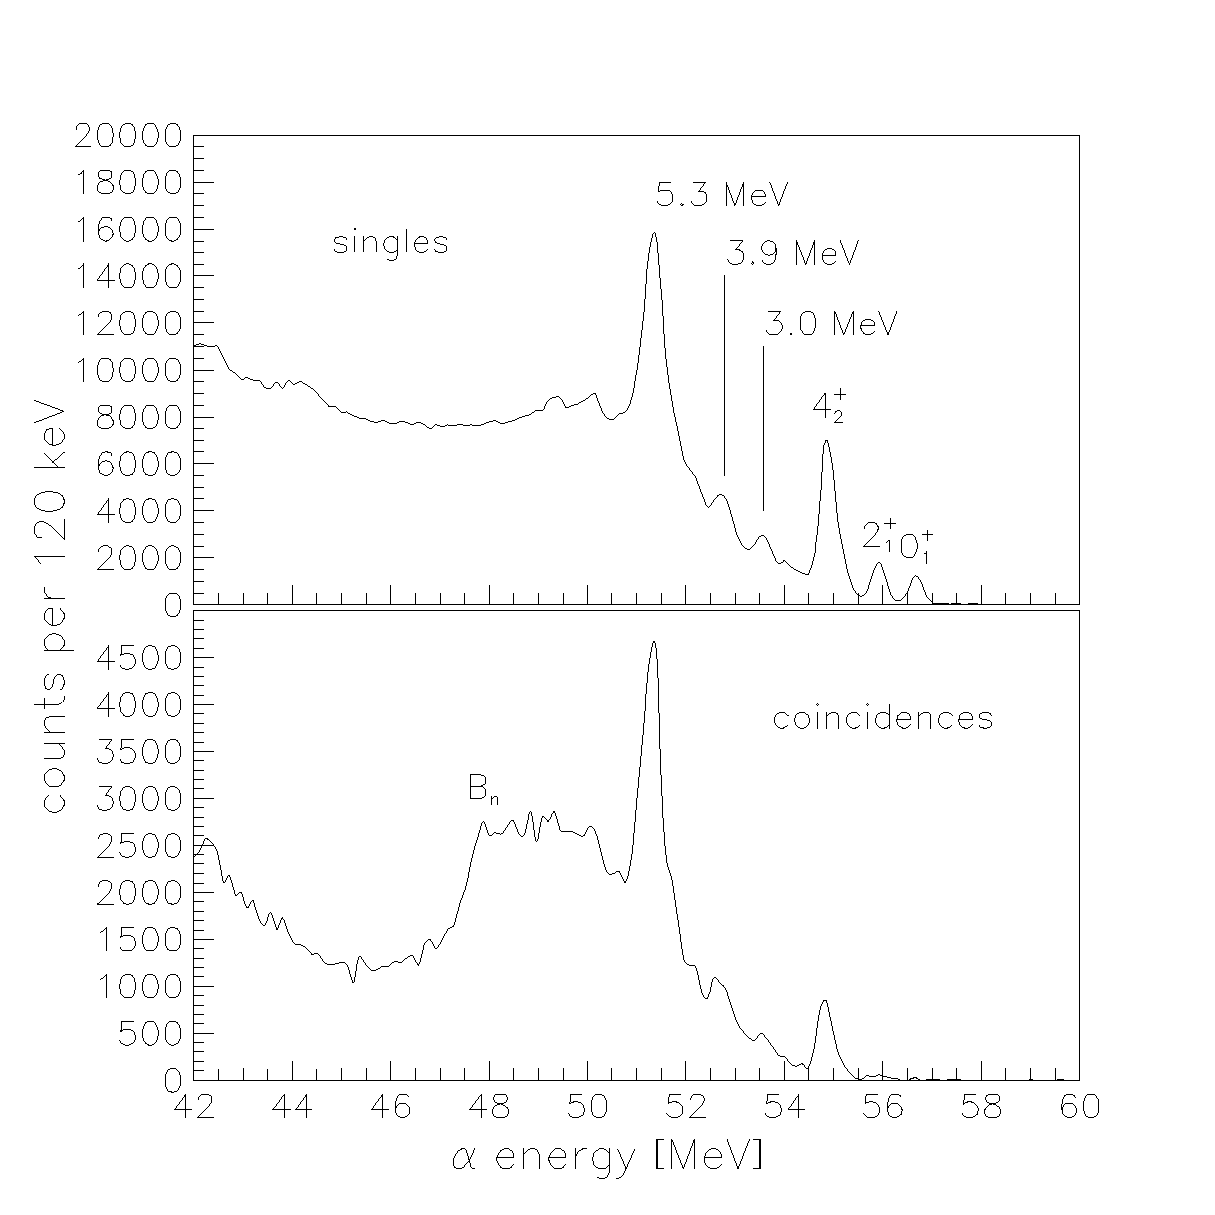
\includegraphics[totalheight=17.9cm]{fig1.eps}
\caption{Single $\alpha$ spectra (upper panel) and in coincidence with $\gamma$
rays (lower panel) from the $^{97}$Mo($^3$He,$\alpha$)$^{96}$Mo reaction. While
the transfer peaks to the first three states are well known from the $(p,d)$ 
reaction, (see Ref.\ \protect\cite{CM73}), the strong transfer into 5.3~MeV has
not been observed before. Subsequently, the 5.3~MeV peak could be confirmed 
(and a similar peak was seen with a $^{95}$Mo target) using the Yale 
spectrograph. We speculate that the $7^+$ member of the coupling of the two 
quasi-particles $(d_{5/2}^{-1}g_{9/2}^{-1})$ \protect\cite{FS73} does not 
fragment very much and is still visible as strong transfer peak in the 
spectrum. Smaller peaks in the spectrum could be fragments of the lower spin 
members from the same quasiparticle configuration. At the neutron binding 
energy $B_n$, the coincidence spectrum shows a step reflecting the lower 
$\gamma$ multiplicity in the decay from low-lying states in $^{95}$Mo which are
populated by neutron emission.}
\label{fig:moraw}
\end{figure}

\clearpage

\begin{figure}\centering
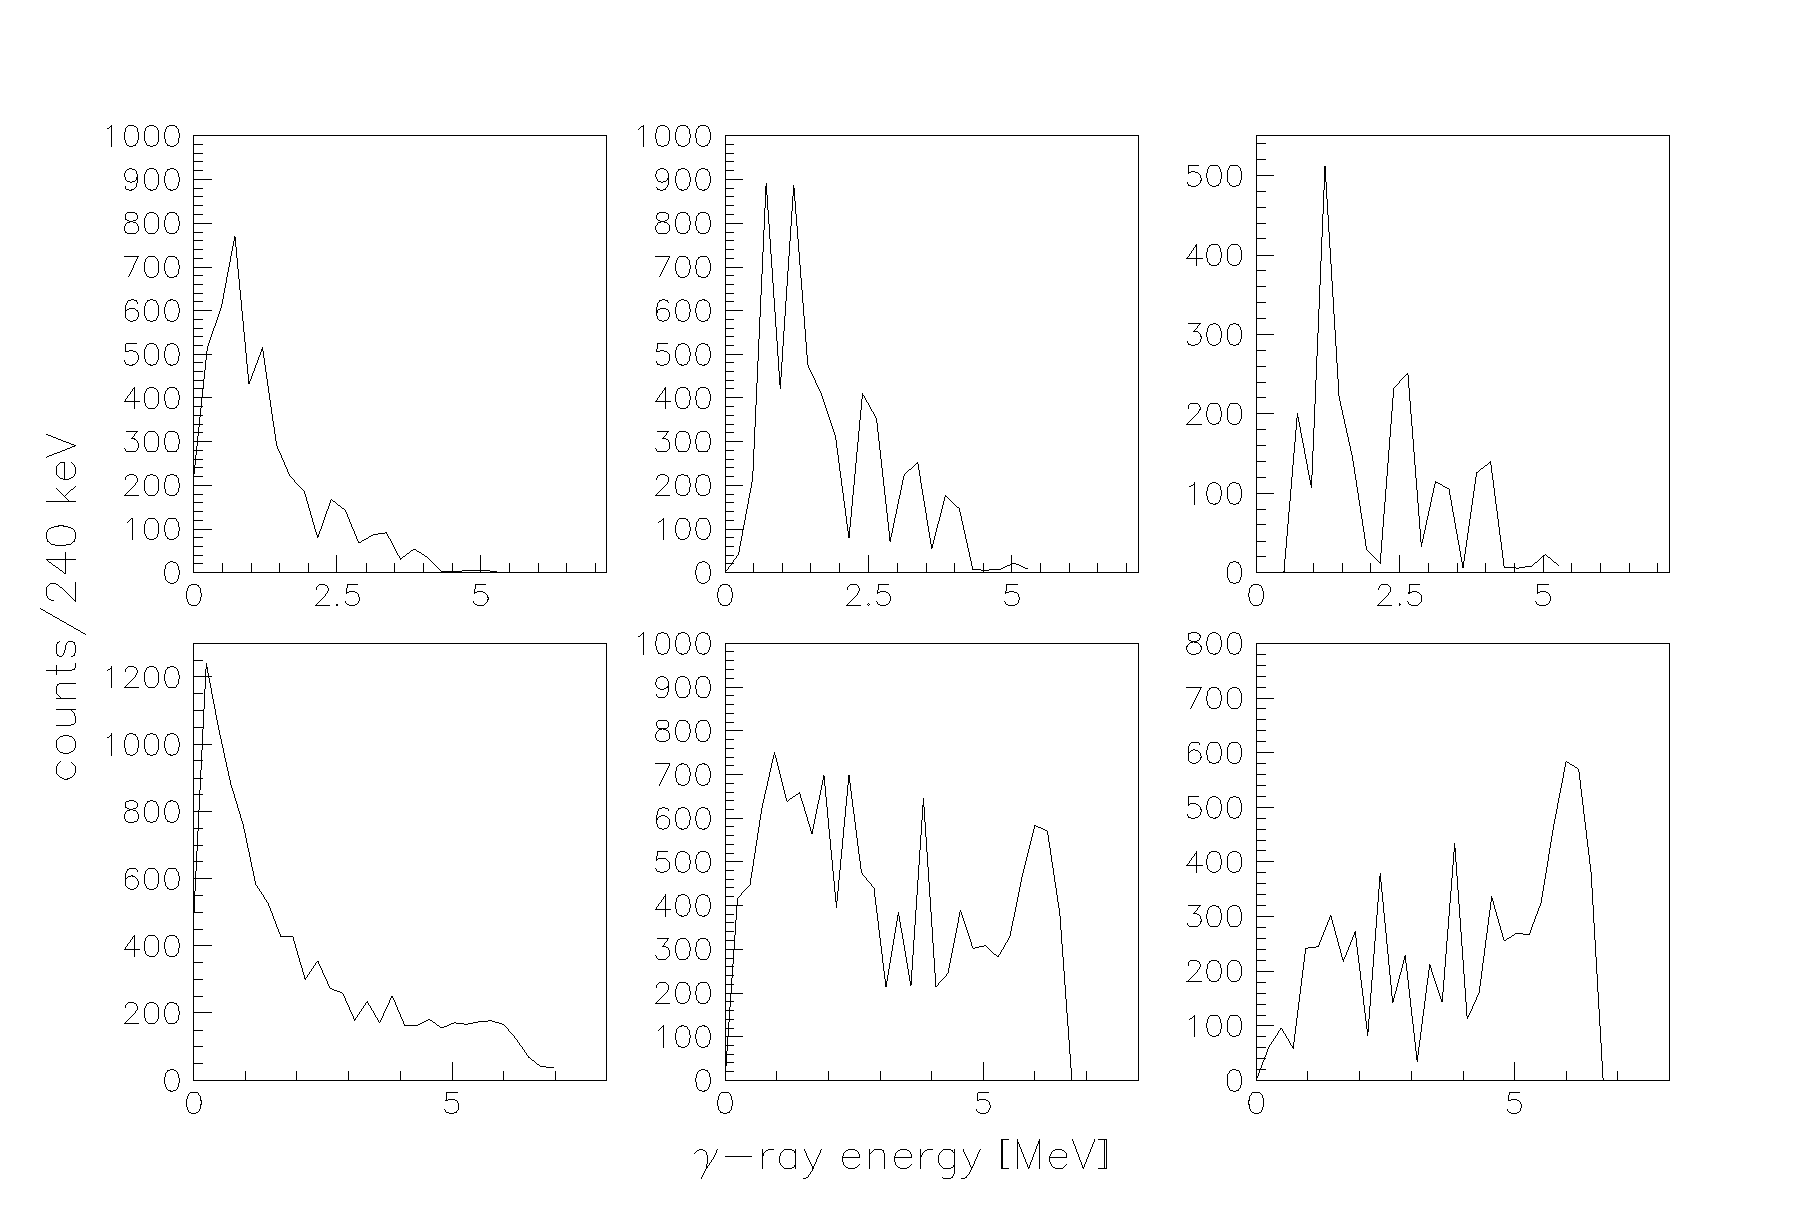
\includegraphics[totalheight=11.9cm]{fig2.eps}
\caption{Raw (left panels), unfolded (center panels), and primary $\gamma$ 
(right panels) spectra from the $^{57}$Fe($^3$He,$\alpha\gamma$)$^{56}$Fe 
reaction at 5~MeV excitation energy (upper panels) and from the  
$^{57}$Fe($^3$He,$^3$He$^\prime\gamma$)$^{57}$Fe reaction at 6.2~MeV excitation
energy (lower panels).}
\label{fig:feraw}
\end{figure}

\clearpage

\begin{figure}\centering
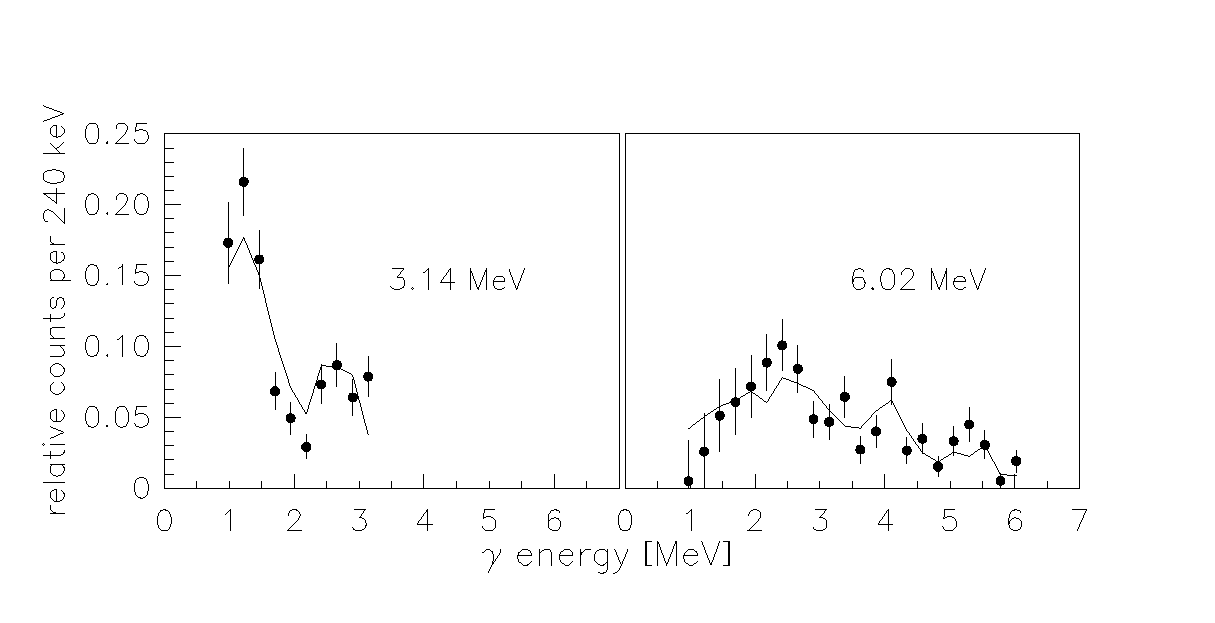
\includegraphics[totalheight=8.9cm]{fig3.eps}
\caption{Experimental primary $\gamma$ spectra (data points with error bars) at
two different initial excitation energies compared to the least $\chi^2$ fit
(solid lines) for the $^{97}$Mo($^3$He,$^3$He$^\prime\gamma$)$^{97}$Mo 
reaction.}
\label{fig:fgmo}
\end{figure}

\clearpage

\begin{figure}\centering
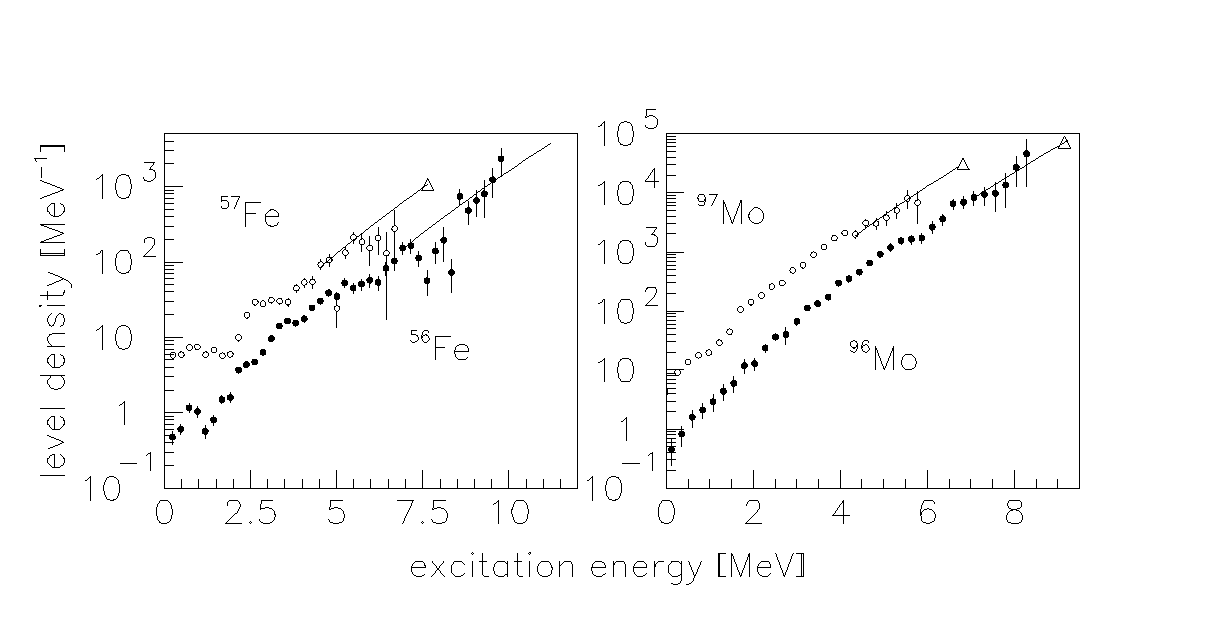
\includegraphics[totalheight=8.9cm]{fig4.eps}
\caption{Experimental level densities for the four nuclei under study. Where
available, level density data from neutron resonance spacings have been added 
(open triangles). The solid lines are the renormalized (forced to go through 
the triangles) level density parameterizations according to von Egidy \sl et 
al.\ \rm \protect\cite{ES88}. Step structures in the level densities are evident at 
2.9~MeV and 1.8~MeV in $^{56}$Fe and $^{57}$Fe and at 2.0~MeV and 1.2~MeV in 
$^{96}$Mo and $^{97}$Mo, respectively. The steps in the iron data are more
pronounced than in the molybdenum data. In the level density of $^{56}$Fe, the 
bumps at 0.8~MeV and 2.0~MeV are due to the first and second excited states.}
\label{fig:levdens}
\end{figure}

\clearpage

\begin{figure}\centering
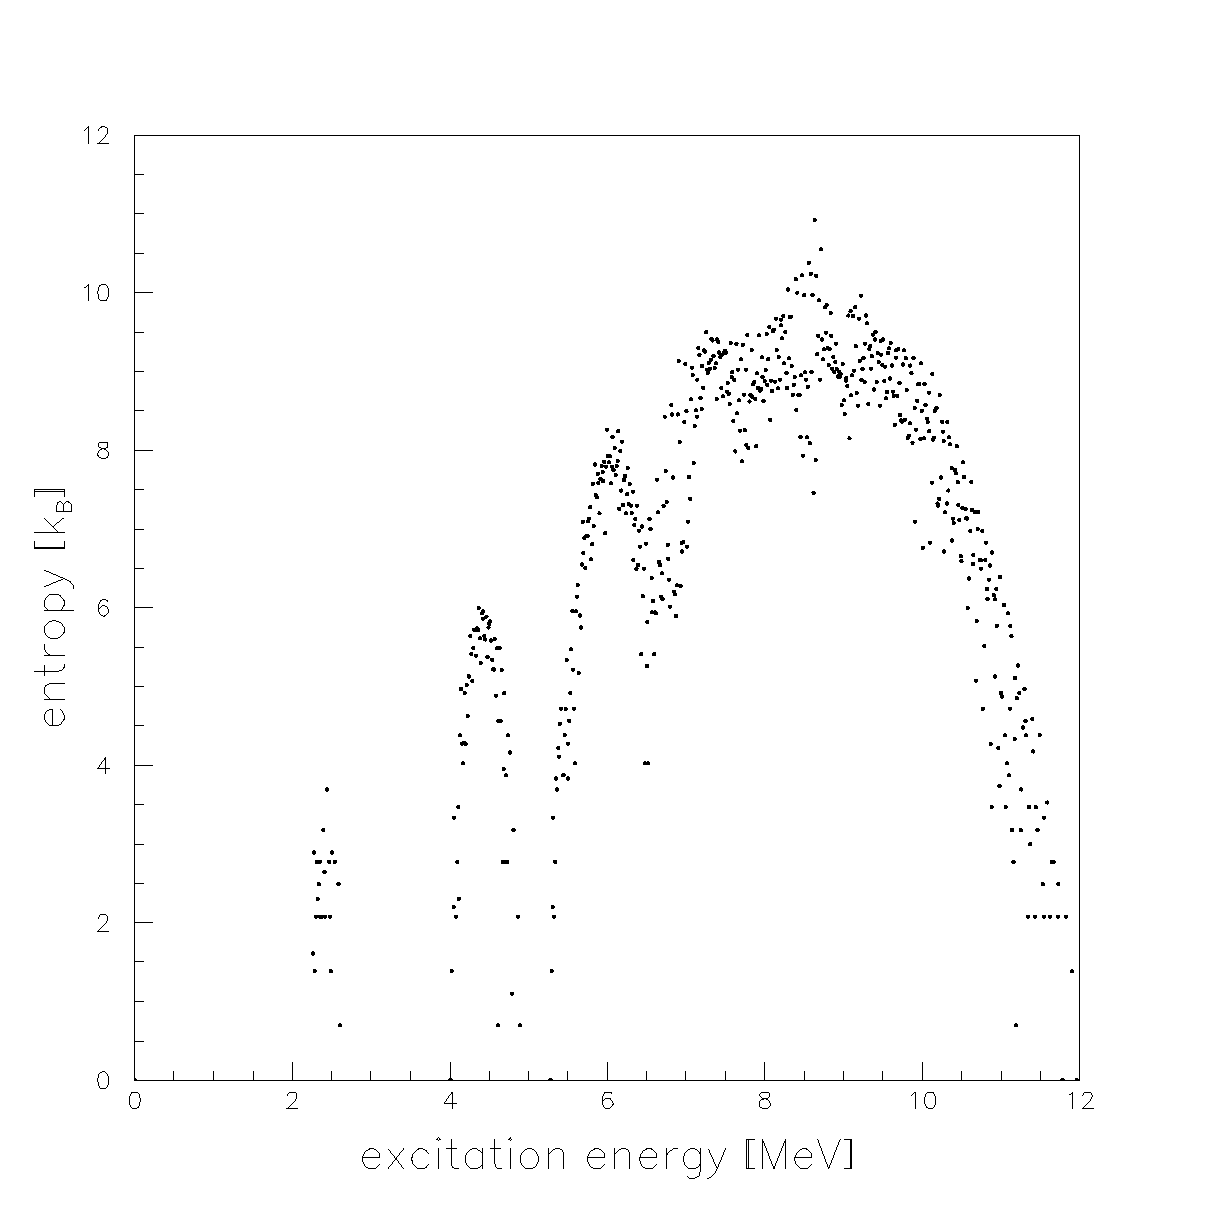
\includegraphics[totalheight=8.9cm]{fig5.eps}
\caption{\bf This figure and figure caption is not finished yet. \rm 
Model calculation using the Hamiltonian of Eq.\ 
(\protect\ref{eq:pairham}) with $\delta=0.5$ (upper panel). The logarithm of 
the level density, i.e., the entropy, is given as function of excitation 
energy. Adding a random two-body interaction of different strength yields
smoothing of the bumps with definite seniority (lower panels, to be calculated
by Calvin. For first results in a smaller space see attached file calvin.pdf.) 
and resembles more the step structures seen in the experimental level densities
of $^{56,57}$Fe and $^{96,97}$Mo.}
\label{fig:calc}
\end{figure}

\end{document}
